\documentclass[11pt, openright]{book}

	% Cover Variables
	\newcommand{\ctitle}{Simulation}
	\newcommand{\cautor}{Lucas Lescure}
	\newcommand{\ctoptitle}{TP Réseau}

	% Header Variables
		\newcommand{\headRE}{\emph{\thepage}}
		\newcommand{\headLE}{\emph{\thesection. \rightmark}}
		\newcommand{\footRE}{}
		\newcommand{\footLE}{}

	% TOC Variables
		\newcommand{\toctitle}{Table of Content}
		\newcommand{\tocchapter}{Chapter}
		\newcommand{\toccount}{3}
  
	% Chapter Variables
		\newcommand{\chvar}{Chapter -}

\usepackage[a4paper, total={16cm, 22.125cm}]{geometry}

% Page Style
\usepackage[]{environ}
% Cover Page 
\usepackage{tikz}
\makeatletter
\def\parsecomma#1,#2\endparsecomma{\def\page@x{#1}\def\page@y{#2}}
\tikzdeclarecoordinatesystem{page}{
    \parsecomma#1\endparsecomma
    \pgfpointanchor{current page}{north east}
    % Save the upper right corner
    \pgf@xc=\pgf@x%
    \pgf@yc=\pgf@y%
    % save the lower left corner
    \pgfpointanchor{current page}{south west}
    \pgf@xb=\pgf@x%
    \pgf@yb=\pgf@y%
    % Transform to the correct placement
    \pgfmathparse{(\pgf@xc-\pgf@xb)/2.*\page@x+(\pgf@xc+\pgf@xb)/2.}
    \expandafter\pgf@x\expandafter=\pgfmathresult pt
    \pgfmathparse{(\pgf@yc-\pgf@yb)/2.*\page@y+(\pgf@yc+\pgf@yb)/2.}
    \expandafter\pgf@y\expandafter=\pgfmathresult pt
}
\makeatother


% Object formatting
\usepackage[12pt]{moresize}
\usepackage[]{anyfontsize}
\usepackage{titlesec}
\usepackage{import}
\usepackage{floatrow}
\usepackage{enumitem}
\usepackage{changepage}
\usepackage[normalem]{ulem}
\usepackage{array}
\newcommand{\ul}[1]{\underline{#1}}

\usepackage[]{chngcntr}
\usepackage{ifthen}
\ifthenelse{\figcountdepth > 1}
  {\counterwithin{figure}{section}\counterwithin{table}{section}}
  {}

\usepackage[format=plain, labelfont=it, textfont=it]{caption}
\makeatletter
\def\@makecaption#1#2{%
    \vskip\abovecaptionskip
    \sbox\@tempboxa{\textit{#1.} #2}

       
   

    \ifdim \wd\@tempboxa >\hsize
        #1. #2\par
    \else
        \global \@minipagefalse
        \hb@xt@\hsize{\hfil\box\@tempboxa\hfil}
    \fi
    \vskip\belowcaptionskip}
\makeatother

\DeclareCaptionFormat{underline}{\uline{#1#2#3}\par}

% Sections
\titleformat{\section}{\fontsize{16}{19.2}\bfseries}{\thesection.}{0.25em}{}
\titleformat{\subsection}{\fontsize{14}{16.8}\bfseries}{\tab\thesubsection.}{0.25em}{}
\titleformat{\subsubsection}{\fontsize{10}{12}}{\uline{\thesubsubsection)\enspace}}{0em}{\uline}





% Geometry

% Typewritting

\setlength{\parskip}{1em}
\setlength{\parindent}{0em}


\newenvironment{items}[3][0pt]
{\def\closesep{#3}
    \vspace{#2}
    \begin{itemize}
        \setlength{\itemsep}{#1}
        \setlength{\topsep}{0pt}
        \setlength{\partopsep}{0pt}}
        {\end{itemize}
    \vspace{\closesep}}

\newenvironment{enum}[3][0pt]
{\defclosesep{#3}
    \vspace{#2}
    \begin{enumerate}
        \setlength{\itemsep}{#1}
        \setlength{\topsep}{0pt}
        \setlength{\partopsep}{0pt}}
        {\end{enumerate}
    \vspace{\closesep}}

\newenvironment{eq}[2]
{\def\closesep{#2}
    \vspace{#1}
    \begin{align*}}
        {\end{align*}
    \vspace{\closesep}}

\newenvironment{lfeq}[2]
{\def\closesep{#2}
    \vspace{#1}
    \begin{flalign*}}
        {\end{flalign*}
    \vspace{\closesep}}
% List Formatting


\NewEnviron{dent}[1]{
    \vspace{-10pt}
    \begin{adjustwidth}{7mm}{}
        \uline{#1}\hspace{2mm}
        \BODY
    \end{adjustwidth}
    \vspace{-10pt}
}


\usepackage[framemethod=tikz]{mdframed}
\newcounter{count_theorem}[section]\setcounter{count_theorem}{0}
\newcommand{\thetheorem}{\arabic{count_theorem}}

\newcounter{count_exercise}[section]\setcounter{count_exercise}{0}
\newcommand{\theexercise}{\arabic{count_exercise}}


\newenvironment{theorem}[1][]{
    \refstepcounter{count_theorem}
    \mdfsetup{
        linecolor=red!30,
        innerbottommargin=10pt,
        linewidth=2pt,
        topline=false,
        bottomline=false,
        rightline=false,
        shadow=true,
        shadowsize=4.5pt,
        frametitlerule=false,
        apptotikzsetting={
                \tikzset{
                    mdfbackground/.append style={
                            left color=red!8,right color=red!3
                        }
                }
            }
    }
    \begin{mdframed}[]\relax
        \ifstrempty{#1}
        {\textbf{Theorem~\thetheorem.} }
        {\textbf{Theorem~\thetheorem.~#1} }
        }
        {\end{mdframed}\vspace{-10pt}
}

\newenvironment{note}{
    \mdfsetup{innertopmargin=5pt,
        linecolor=gray!30,
        linewidth=2pt,
        topline=false,
        bottomline=false,
        rightline=false,
        frametitleaboveskip=0pt,
        shadow=false,
        shadowsize=4pt,
        frametitlerule=false,
        apptotikzsetting={
                \tikzset{
                    mdfbackground/.append style={
                            left color=gray!8,right color=gray!3
                        }
                }
            }
    }
    \begin{mdframed}[]\relax
        \textbf{Note. }
        }
        {\end{mdframed}\vspace{-10pt}
}

\newenvironment{example}{
    \mdfsetup{innertopmargin=5pt,
        linecolor=green!30,
        linewidth=2pt,
        topline=false,
        bottomline=false,
        rightline=false,
        frametitleaboveskip=0pt,
        shadow=false,
        shadowsize=4pt,
        frametitlerule=false,
        apptotikzsetting={
                \tikzset{
                    mdfbackground/.append style={
                            left color=green!7,right color=green!2
                        },
                    mdfframetitlebackground/.append style={
                            left color=green!7,right color=green!2
                        }
                }
            }
    }
    \begin{mdframed}[]\relax
        \textbf{Example. }
        }
        {\end{mdframed}\vspace{-10pt}
}


\usetikzlibrary{calc,arrows}

\tikzset{
    excursus arrow/.style={%
            line width=2pt,
            draw=gray!40,
            rounded corners=2ex,
        },
    excursus head/.style={
            fill=white,
            font=\bfseries\sffamily,
            text=gray!80,
            anchor=base west,
        },
    excursus line/.style={%
            line width=2pt,
            draw=gray!40,
            rounded corners=2ex,
        }
}

\newenvironment{exercise}[1][]{%
    \refstepcounter{count_exercise}
    \mdfsetup{
        singleextra={
                \path let \p1=(P), \p2=(O) in (\x2,\y1) coordinate (Q);
                \path let \p1=(Q), \p2=(O) in (\x1,{(\y1-\y2)/2}) coordinate (M);
                \path [excursus line] ($(O)+(5em,0ex)$) -| (M) |- ($(Q)+(20em,0ex)$);
                \node [excursus head] at ($(Q)+(2.5em,-0.75pt)$) {\ifstrempty{#1}{Exercise \theexercise}{Exercise \theexercise:~#1}};},
        firstextra={
                \path let \p1=(P), \p2=(O) in (\x2,\y1) coordinate (Q);
                \path [excursus arrow,-to] (O) |- ($(Q)+(12em,0ex)$) .. controls +(0:16em) and +(185:6em) .. ++(23em,2ex);},
        middlelinewidth=2.5em,middlelinecolor=white,
        hidealllines=true,topline=true,
        innertopmargin=0.5ex,
        innerbottommargin=2.5ex,
        innerrightmargin=2pt,
        innerleftmargin=2ex,
        skipabove=0.87\baselineskip,
        skipbelow=0.62\baselineskip,
    }
    \begin{mdframed}[]\relax}
        {\end{mdframed}\vspace{-10pt}
}

% Functions and Data Plotting
\usepackage{subfig,wrapfig,adjustbox,multirow}


% Plotting Style
\usepackage{graphicx,pgfplots}
\usetikzlibrary{arrows}
\usetikzlibrary {patterns,patterns.meta}
\usepgfplotslibrary{fillbetween}
\pgfplotsset{compat=1.18}

\usepgfplotslibrary{units}
% Logarithmic Scale
\pgfplotsset{
    log x ticks with fixed point/.style={
            xticklabel={
                    \pgfkeys{/pgf/fpu=true}
                    \pgfmathparse{exp(\tick)}%
                    \pgfmathprintnumber[fixed relative, precision=3]{\pgfmathresult}
                    \pgfkeys{/pgf/fpu=false}
                }
        }
}


% Mathematics

% Formatting
\usepackage{amsmath}
\usepackage{esvect}
\usepackage{amsfonts}
\usepackage{tasks,environ}
\usepackage{xargs}
\usepackage{esint}
\usepackage[]{listings}


\usepackage[english]{babel}
\usepackage{amsthm}
%\newtheorem{theorem}{Theorem}
%\newtheorem{proof}{Proof}



%Custom Shortcuts
\newcommand{\eqi}{\Leftrightarrow}
\newcommand{\lr}[1]{\left( #1 \right)}
\newcommand{\limit}[1]{\displaystyle{\lim_{#1}}}
\newcommand{\tab}{\hspace*{7mm}}
\newcommand{\ds}[1]{\displaystyle{#1}}
\newcommand{\floor}[1]{\lfloor #1 \rfloor}
\newcommand{\R}{\mathbb{R}}
\newcommand{\N}{\mathbb{N}}
\newcommand{\Z}{\mathbb{Z}}
\newcommand{\C}{\mathbb{C}}
\newcommand{\K}{\mathbb{K}}
\newcommand{\F}{\mathcal{F}}
\newcommand{\M}{\mathcal{M}}
\renewcommand{\l}{\lambda}
\newcommand{\seg}[1]{\overline{\rm {#1}}}
\newcommand{\Int}{\int\limits}
\newcommand{\ex}{\tab \uline{Example :}\hspace{0.2cm} }
\newcommand{\vard}{\partial}
\newcommand{\Q}{\mathcal{Q}}
\newcommand{\Vect}{\operatorname{Vect}}
\newcommand{\rg}{\operatorname{rg}}
\renewcommand{\dim}{\operatorname{dim}}
\renewcommand{\Re}{\operatorname{Re}}
\renewcommand{\Im}{\operatorname{Im}}
\renewcommand{\P}{\mathcal{P}}
\newcommand{\blr}[1]{\left\{#1\right\}}
\newcommand{\linecenter}[1]{\par\vspace{2mm} \centerline{#1}\par\vspace{-2mm}}
\newcommand{\dd}{\textrm{d}}
\newcommand{\supp}{\operatorname{Supp}}
\renewcommand{\vec}{\overrightarrow}
\renewcommand{\epsilon}{\varepsilon}

% Matrix Configurations

\makeatletter
\renewcommand*\env@matrix[1][*\c@MaxMatrixCols c]{%
    \hskip -\arraycolsep
    \let\@ifnextchar\new@ifnextchar
    \array{#1}}
\makeatother


% Colors
\usepackage{xcolor}
\newcommand{\blu}{\color{blue}}
\newcommand{\Red}{\color{red}}
\newcommand{\blac}{\color{black}}

\newcommand{\red}[1]{\textcolor{red}{#1}}

\usepackage{xcolor,xspace}
\usepackage{breqn}


% Headings  
\usepackage[Glenn]{fncychap}
\ChNumVar{\fontsize{40}{42}}
\ChTitleVar{\Large\sc}
\ChNameVar{\Large\sc}
\setlength\headheight{14.5pt}
\renewcommand\FmN[1]{\chvar}



\usepackage{fancyhdr}
\usepackage{ragged2e}

% Header & Footers
\renewcommand{\chaptermark}[1]{\markboth{#1}{#1}}
\renewcommand{\sectionmark}[1]{
    \markright{ #1}
}
\pagestyle{fancy}
\fancyhf{}
\fancyhead[LE,RO]{\headLE}
\fancyhead[RE,LO]{\headRE}
\fancyfoot[LE,RO]{\footLE}
\fancyfoot[RE,LO]{\footRE}
\renewcommand{\headrulewidth}{0.5pt}
\fancyheadoffset{1cm}

\fancypagestyle{plain}{%
    \fancyhf{} % clear all header and footer fields
    \fancyfoot[LE, RO]{\footLE}
    \renewcommand{\headrulewidth}{0pt}
    \renewcommand{\footrulewidth}{0pt}}


\fancypagestyle{nohead}{%
    \fancyhf{} % clear all header 
    \fancyfoot[LE, RO]{\footLE}
    \fancyfoot[LO, RE]{\footRE}}

    \fancypagestyle{head}{%
    \fancyhf{} % clear all header 
    \fancyhead[LE,RO]{\headLE}
\fancyhead[RE,LO]{\headRE}
\renewcommand{\headrulewidth}{0.5pt}
\fancyheadoffset{1cm}
    }


\fancypagestyle{bib}{%
    \fancyhf{} % clear all header and footer fields
    \fancyhead[CE, CO]{}
    \fancyfoot[LE, RO]{\footLE}
    \fancyfoot[LO, RE]{Bibliographie}}

% Table of Contents

\renewcommand*\thechapter{\arabic{chapter}} %Usually Roman
\renewcommand*\thesection{\arabic{section}}
\renewcommand*\thesubsubsection{\thesubsection.\alph{subsubsection}}
\makeatletter
\@removefromreset{section}{chapter}
\makeatother


% Table of Contents

\usepackage{titletoc}
\usepackage{ erewhon,cabin}
\usepackage[linktoc=all]{hyperref}
\renewcommand*\contentsname{\centerline{\toctitle}}

\setcounter{secnumdepth}{3}
\setcounter{tocdepth}{\toccount}

\usepackage[subfigure]{tocloft}
\setlength\cftparskip{0pt}

\usepackage{etoolbox}
\makeatletter
\pretocmd{\chapter}{\addtocontents{toc}{\protect\addvspace{5\p@}}}{}{}
\pretocmd{\section}{\addtocontents{toc}{\protect\addvspace{-10\p@}}}{}{}
\pretocmd{\subsection}{\addtocontents{toc}{\protect\addvspace{1\p@}}}{}{}
\makeatother


% Chapter Style
\titlecontents{chapter}
[11em]
{\bigskip}
{\bfseries\textsc\tocchapter~\textsc\thecontentslabel : \textsc}
{\hspace*{-5.5em}\textbf}
{\titlerule*[1pc]{ }}[\smallskip]

% Section Style
\titlecontents{section}
[0em] % i
{\bigskip\bfseries}
{\fontsize{11}{13.2}\bfseries\uline{\thecontentslabel.\enspace}\uline}
{\hspace*{-4em}\textbf}
{\hspace{0.5pt}\uline{\hspace*{\fill}}\contentspage}

% Subsection Style
\titlecontents{subsection}
[2em] % i
{\smallskip\bfseries}
{\fontsize{10}{12}\bfseries\thecontentslabel.\enspace}
{\hspace*{-4em}}
{\titlerule*[0.5pc]{.}\contentspage}

% Subsubsection Style
\titlecontents{subsubsection}
[4em] % i
{\smallskip}
{\fontsize{10}{12}\thecontentslabel)\enspace}
{\hspace*{-4em}}
{\titlerule*[0.5pc]{.}\contentspage}










	% figure support
	\usepackage{import}
	\usepackage{xifthen}
	\pdfminorversion=7
	\usepackage{pdfpages}
	\usepackage{transparent}
	\newcommand{\incfig}[1]{%
			\def\svgwidth{\columnwidth}
			\import{./figures/}{#1.pdf_tex}
	}

	\pdfsuppresswarningpagegroup=1

\begin{document}
% Spacing
% Section Spacing
\titlespacing\section{0pt}{3pt plus 2pt minus 2pt}{6pt plus 2pt minus 1pt}
\titlespacing\subsection{0pt}{0pt plus 1pt minus 1pt}{0pt plus 3pt minus 1pt}
\titlespacing\subsubsection{0pt}{0pt plus 0pt minus 0pt}{0pt plus 2pt minus 0pt}

\usetikzlibrary{shadows}

\newgeometry{left=2.5cm, width=16cm, bottom=2.5cm, top=2.5cm}






% Cover
% Cover
\definecolor{ccolor1}{RGB}{236,145,143}
\definecolor{ccolor2}{RGB}{131,168,192}
\definecolor{ccolor3}{RGB}{182,227,150}
\definecolor{ccolor4}{RGB}{171,206,145}

\usetikzlibrary{fadings}

\begin{titlepage}
    \newgeometry{top=1cm, width=21cm, bottom=1cm}

    \begin{tikzpicture}[remember picture,overlay,every node/.style={anchor=center}]

        \coordinate (Center) at (page cs: 0,-0.5);
        %F4E Logo
        \begin{scope}[scale = 1.5]
            \foreach \angle in {0,30,...,330} {
                    \filldraw[orange!50!yellow,line width=0.01pt,shift=(Center)] (\angle:3.8637) -- (\angle+30:3.8637) -- (0,0) -- (\angle:3.8637);
                    \draw[white, line width = 7pt,shift=(Center)] (\angle:2cm) arc (\angle-60:\angle:2cm);
                    \draw[white, line width = 7pt,shift=(Center)] (\angle+30:2cm) arc (\angle+90:\angle+30:2cm);
                }
            % Outer delimiter
            \foreach \angle in {15,45,...,345} {
                    \filldraw[white, line width = 7pt,shift=(Center)] (\angle:3.8637cm) arc (\angle-15:\angle+45:2cm) arc (\angle+15:\angle-15:2cm) arc (\angle+45:\angle+15:2cm);
                }
            % Inner delimiter
            \foreach \angle in {15,45,...,345} {
                    \filldraw[white, line width = 7pt,shift=(Center)] (\angle:1.0353cm) arc (\angle-75:\angle-45:2cm) arc (\angle+75:\angle+105:2cm) -- (0,0) -- (\angle:1.0353cm);
                }
            % Stars
            \foreach \angle in {0,30,...,330} {
                    \fill[orange!50!yellow,shift=(Center)] (\angle:1.03527cm) -- ++ (231:0.175) -- ++ (33:0.35) -- ++ (177:0.35) -- ++ (321:0.35) -- ++ (105:0.35) -- ++ (249:0.35) -- ++ (33:0.35);
                }
        \end{scope}

        \node[opacity =0.07, inner sep=0pt, anchor=east] at (current page.east){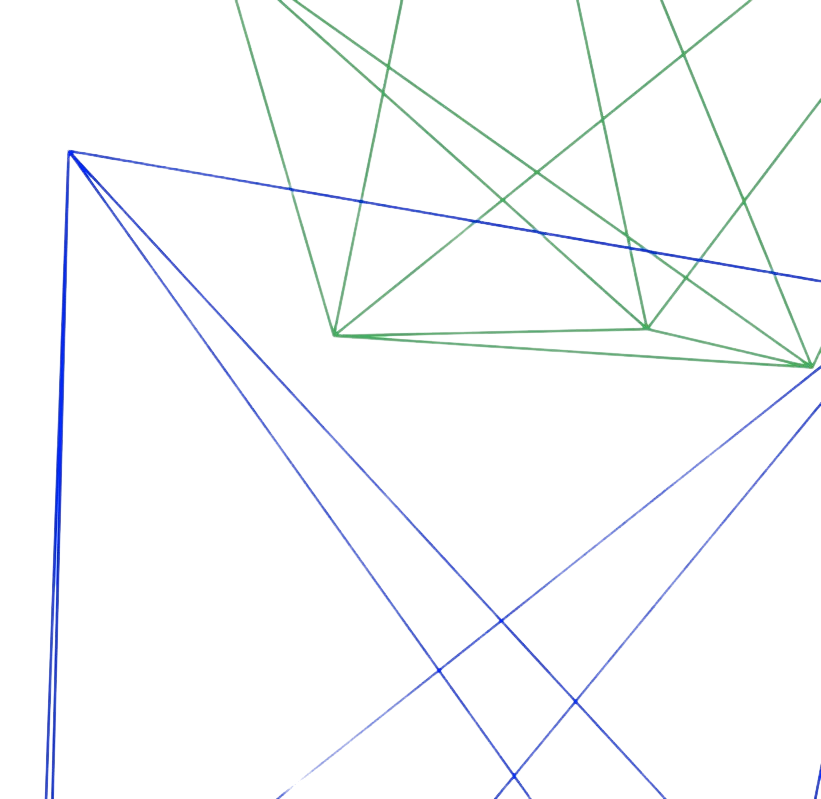
\includegraphics[width=0.5\paperwidth,height=\paperheight]{/root/.config/latex-utils/logos/invert1.png}};

        \node[opacity=0.07,inner sep=0pt, anchor=north west] at (current page.north west){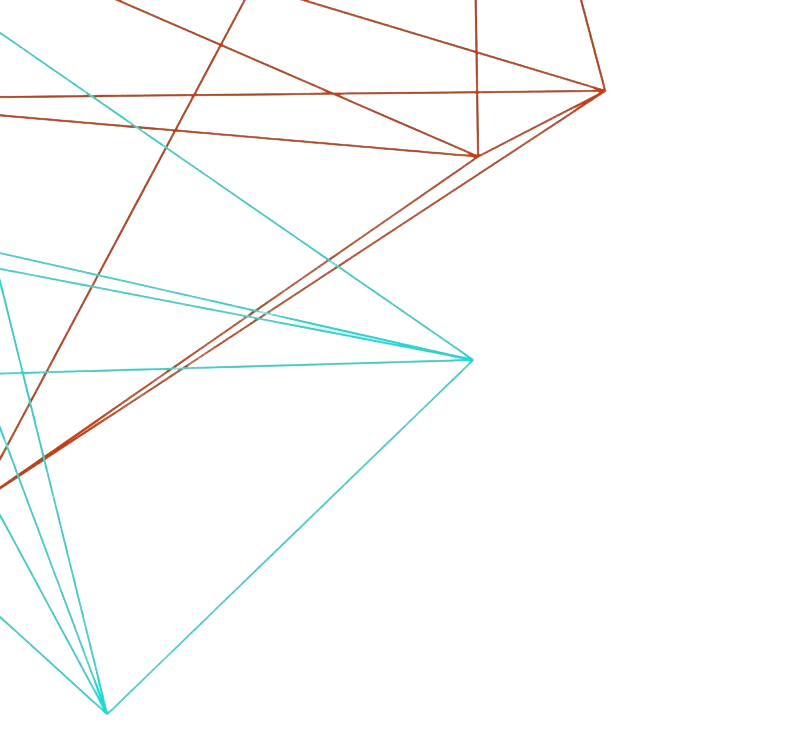
\includegraphics[width=0.5\paperwidth,height=0.5\paperheight]{/root/.config/latex-utils/logos/invert3.png}};




        \node at (page cs:0,0.345) {\Large\textsc{High School Observation and Learning Internship}};
        \node at (page cs:0,0.875) {\Large\bfseries\textsc{Observation Internship}};
        \node at (page cs:0,0.925) {\LARGE\bfseries\textsc{Lycée Français de Barcelone}};

        \node at (page cs:0.5,0) {\Large\textsc{Cyril Lescure - Pedagogical Tutor}};








        %\node[opacity=0.15, inner sep=0pt, anchor=south west] at (current page.south west){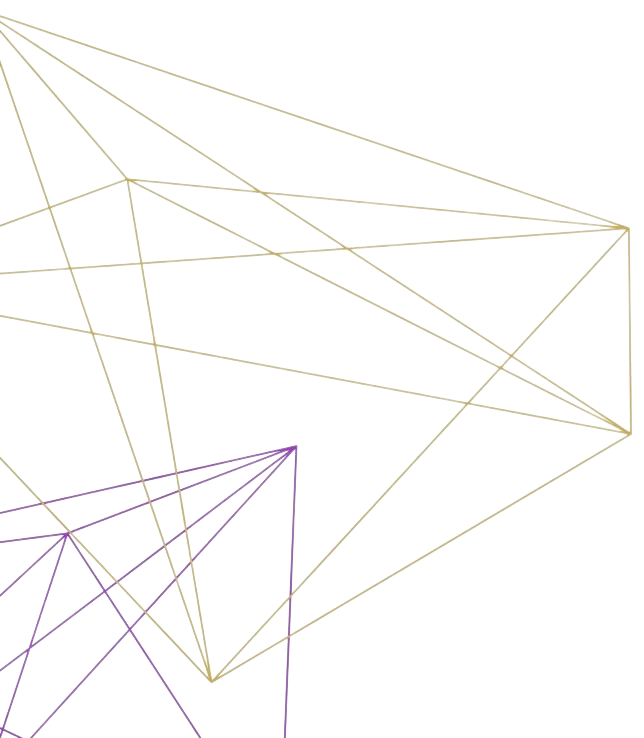
\includegraphics[width=0.5\paperwidth,height=0.5\paperheight]{/root/.config/latex-utils/logos/invert2.png}};

        \node at (page cs:0,0.5) {\fontsize{28}{28.8}\textbf{\ctoptitle}};
        \node at (page cs:0,0.425) {\fontsize{28}{28.8}\textbf{\ctitle}};
        \draw (page cs:0.5,0.375) -- (page cs:-0.5,0.375);
        \node at (page cs:0,0.245) {\LARGE\textsc{\cautor}};
        \node at (page cs:0,0.310) {\Large\textsc{03.06.2019 - 07.06.2019}};


    \end{tikzpicture}
\end{titlepage}


\newgeometry{width=18.625cm, bottom=2cm, top=2cm}

\tikz[remember picture, overlay] \node[opacity=0.3,inner sep=0pt, anchor=north east] at (current page.north east){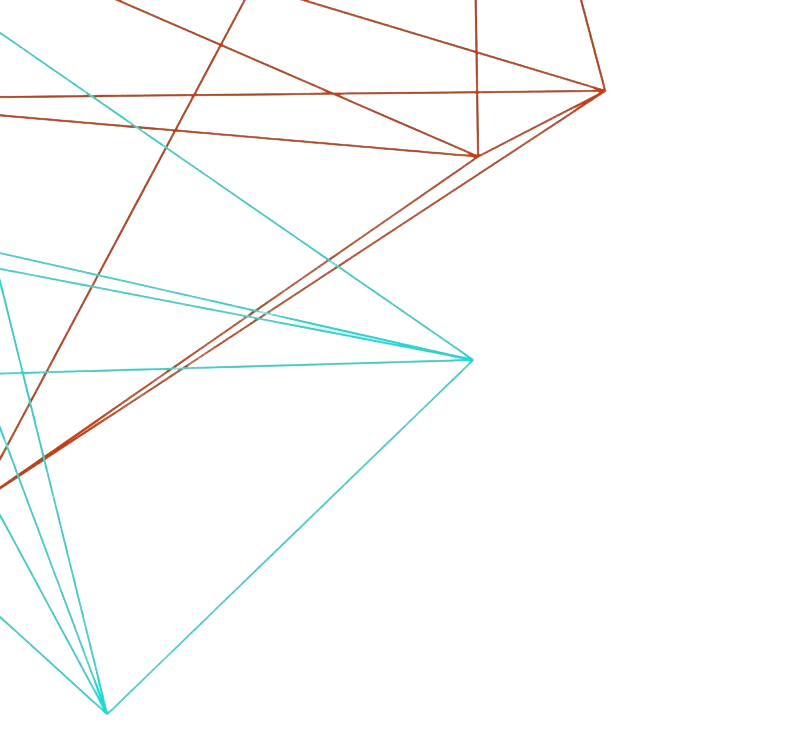
\includegraphics[angle=-90,origin=c,width=0.5\paperheight,height=0.5\paperwidth]{/root/.config/latex-utils/logos/invert3.png}};
\tikz[remember picture,overlay] \node[opacity=0.3,inner sep=0pt, anchor=south east] at (current page.south east){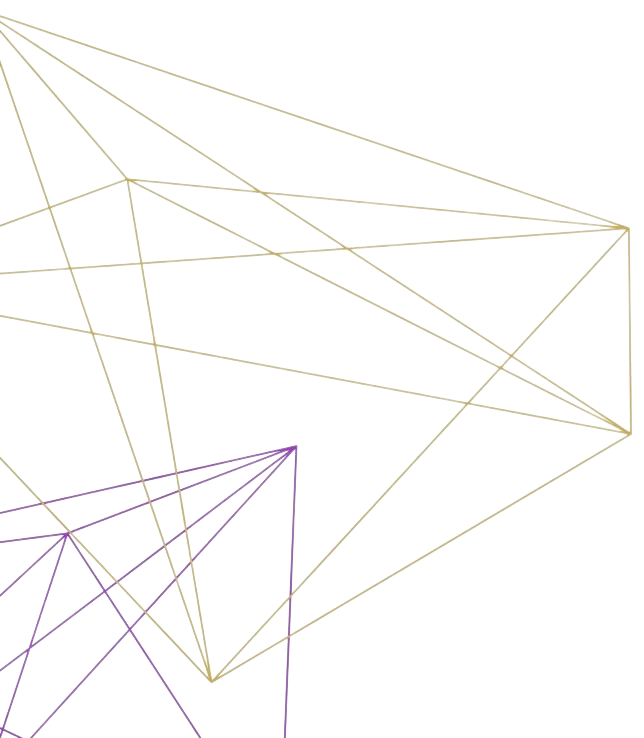
\includegraphics[angle=90,width=0.5\paperwidth,height=0.5\paperheight]{/root/.config/latex-utils/logos/invert2.png}};

\tableofcontents





\newpage

\section{Exercise 1: Transmission Ethernet}

\begin{dent}{Q1 :} Quels types de câbles peut-on utiliser?\\
	Nous avons le choix entre 4 types de cables différents: 
	\begin{items}{-15pt}{-15pt}
		\item Paire de cables torsadées droit 
		\item Paire de cables torsadées croisé
		\item Câble coaxial
		\item Ligne telecom
	\end{items}
	On voit qu'avec la paire de cables torsadée droit, et ligne telecom il n'y a pas de transmission entre les deux machines, alors que pour la paire de cable torsadées croisé et le cable coaxial il y a une transmission entre les deux machines.
\end{dent}

\begin{dent}{Q2 :} Que se passe-t-il quand un système émet vers l'autre(broadcast-unicast)? Que se passe-t-il quand les 2 systèmes émettent l'un vers l'autre\\
	\begin{enum}{-15pt}{-15pt}
		\item[a.] Lorsqu'une machine émet une trame, celle-ci est émise à la deuxième machine dans son réseau. De même avec une transmission \texttt{unicast}.
		\item[b.] Avec une paire torsadé croisé on voit que les deux trames sont envoyés sur un fil différent il n'y a pas de collision de la trame. Avec une paire de cable coaxial on voit que ces deux trames sont transmises sur un même fil, il y a donc une collision. Les deux machines attendes un moment aléatoire avant que l'une d'elle ne renvoi la trame. S'il n'y a pas encore une collision, la première trame est transmise en premier, puis une fois finie, la deuxième trame est envoyée. 
	\end{enum}
\end{dent}

\begin{dent}{Q3 :} Après avoir vider les tables ARP de chaque machine, on effectue un ping de \texttt{st1} à \texttt{st2}\\
	Quelles sont les trames mises en oeuvre lorsque \texttt{st1} fait un ping vers \texttt{st2}?\\
	Quelle est la différence si on renouvelle ce ping (cache ARP)?
	
	\begin{enum}{-15pt}{-15pt}
		\item[a.] \texttt{st1} verifie sa table de routage pour savoir où envoyer la trame. Ensuite il envoi une requête ARP en broadcast vers tout les appareil. Quand \texttt{st2} reçois la trame il cherche l'IP source dans son cache, puisqu'elle n'y est pas, il rajoute l'IP avec l'adresse mac associé. Il examine ensuite la trame pour savoir si elle lui est destinée puis après avoir traité la trame il la renvoi une réponse ARP à la machine \texttt{st1}. Celle-ci ne reconnais pas la source et l'ajoute donc dans son cache. Après traitement du signal elle envoi une trame IP "\texttt{echo}" qui ping la machine \texttt{st2}, qui la renvoi ensuite après avoir traité et reconnue l'adresse source. Le paquet \texttt{EchoResponse} est lu par \texttt{st1} il sait donc que sont ping à bien été transmis. 
		\item[b.] Quand leur table ARP est déjà remplie, c'est à dire que les deux machine se connaissent, il n'y a pas de requête ARP, on passe directement à l'envoi de la trame \texttt{echo} par transmission IP.
	\end{enum}
\end{dent}

\section{Exercise 2 : Plusieurs systèmes raccordés par un HUB}

\begin{dent}{Q1 :} Quel type de câble peut-on utiliser?\\
	On ne peut utiliser que la paire de cable torsadée droit. Ce qui est logique car en présence d'un HUB on ne passe plus par une connection entre deux appareil de même type, la liaison se fait entre de appareils de type différent. 
\end{dent}

\begin{dent}{Q2 \& Q3 :} Quels systèmes reçoivent la trame(\texttt{broadcast}/\texttt{unicast}), et lesquelles la traitent?
	
	Lorsque l'on envoi une trame en \texttt{broadcast}, cette trame atteint toutes les machines liés au HUB, et elle est lu par tout le monde. En \texttt{unicast}, tout le monde reçois mais seulement la machine destinataire lit le message transmis.     
\end{dent}

\begin{dent}{Q4 :}
	Lorsque l'on a deux machines qui envoi simultanément une trame, lorsque les deux trames atteignent le HUB, il y a collision sur toutes les autres transmission. On attend un temps aléatoire avant que l'une n'envoi sa trame, s'il n'y a pas encore de collision alors la deuxième enverra sa trame une fois que la première se fasse traiter. 
\end{dent}


\newpage

\section{Exercise 3 : Plusieurs systèmes raccordés par un SWITCH}

\begin{dent}{Q1 :} Quel type de cable faut-il utiliser?\\
	Comme dans l'exercise précédent on doit utiliser le cable torsadée droit
\end{dent}

\begin{dent}{Q2 :} Différence entre "on the fly" et "store and forward"
	\begin{enum}{-15pt}{-15pt}
		\item[a.] Lorsque l'on met le switch en mode "on the fly" on voit que les trames sont à la fois routés vers le réseaux et sauvegardées en mémoire par la switch pour être sur qu'il n'y ai pas de collision sur les transmissions.  
		\item[b.] En mode "store and forward" il attend d'avoir reçu la trame entièrement avant de les renvoyer sur les machines du réseau, on évite aussi les collision entre les trames. 
	\end{enum}
\end{dent}

\begin{dent}{Q3 :} On affiche la table MAC/Port du switch :
	\begin{figure}[ht]
		\centering
		\begin{tabular}{|c|c|c|}
			\hline
			Adresse & Port & TTL   \\
			\hline
			MAC01   & 1    & Elevé \\
			\hline
			MAC02   & 2    & Elevé \\
			\hline
			MAC03   & 3    & Elevé \\
			\hline
			MAC04   & 4    & Elevé \\
			\hline
		\end{tabular}
		\caption{\ul{Table MAC/Port SWITCH}}
	\end{figure}
\end{dent}

\begin{dent}{Q4 \& Q5 :} Que fait le switch?\\
	Le switch transmet directement d'une machine à l'autre agissant comme un pont, seulement la machine destinée reçoit la trame.
	
\end{dent}


\begin{dent}{Q7 :} On affiche la table MAC/Port suite aux 3 transmissions:
	\begin{figure}[ht]
		\centering
		\begin{tabular}{|c|c|c|}
			\hline
			Addresse & Port & TTL   \\
			\hline
			MAC01    & 1    & Élevé \\
			\hline
			MAC03    & 3    & Moyen \\
			\hline
		\end{tabular}
		\caption{\ul{Table MAC/Port SWITCH}}
	\end{figure}
\end{dent}

\begin{dent}{Q8 :} Quel est le rôle de la découverte du réseau
	La découverte du réseau permet directement de connaitre tout les appareils branchés sur le switch, sans devoir envoyer une trame à chacun pour remplir la table MAC/Port.
\end{dent}

\newpage

\section{Exercise 4 : Système Complet}

\begin{dent}{Q1 :}
	On relève les IP de \texttt{st1} et \texttt{st5} :
	\begin{items}{-15pt}{-15pt}
		\item \texttt{st1} : 194.214.131.1 (Masque : 255.255.255.0) c'est une classe C
		\item \texttt{st5} : 161.3.1.5 (Masque : 255.255.0.0) c'est une classe B
	\end{items}
\end{dent}


\begin{figure}[ht!]
	\centering
	\begin{tabular}{|l|l|l|l|l|}
		\hline
		No. & Destination     & Masque          & Passerelle    & Interface     \\
		\hline
		1   & 194.214.131.1   & 255.255.255.255 & 194.214.131.1 & 194.214.131.1 \\
		\hline
		2   & 194.214.131.0   & 255.255.255.0   & 194.214.131.1 & 194.214.131.1 \\
		\hline
		3   & 194.214.131.255 & 255.255.255.255 & 194.214.131.1 & 194.214.131.1 \\
		\hline
		4   & 0.0.0.0         & 0.0.0.0         & 194.214.131.4 & 192.214.131.1 \\
		\hline
	\end{tabular}
	\caption{\ul{Table routage de \texttt{st1}}}
\end{figure}

\begin{figure}[ht!]
	\centering
	\begin{tabular}{|l|l|l|l|l|}
		\hline
		No. & Destination   & Masque          & Passerelle & Interface \\
		\hline
		1   & 161.3.1.5     & 255.255.255.255 & 161.3.1.5  & 161.3.1.5 \\
		\hline
		2   & 161.3.0.0     & 255.255.0.0     & 161.3.1.5  & 161.3.1.5 \\
		\hline
		3   & 161.3.255.255 & 255.255.255.255 & 161.3.1.5  & 161.3.1.5 \\
		\hline
		4   & 0.0.0.0       & 0.0.0.0         & 161.3.1.4  & 161.3.1.5 \\
		\hline
	\end{tabular}
	\caption{\ul{Table routage de \texttt{st5}}}
\end{figure}

\begin{figure}[ht!]
	\centering
	\begin{tabular}{|l|l|l|l|l|}
		\hline
		No. & Destination     & Masque          & Passerelle    & Interface     \\
		\hline
		1   & 161.3.1.4       & 255.255.255.255 & 161.3.1.4     & 161.3.1.4     \\
		\hline
		2   & 161.3.0.0       & 255.255.0.0     & 161.3.1.4     & 161.3.1.4     \\
		\hline
		3   & 161.3.255.255   & 255.255.255.255 & 161.3.1.4     & 161.3.1.4     \\
		\hline
		4   & 194.214.131.4   & 255.255.255.255 & 194.214.131.4 & 194.214.131.4 \\
		\hline
		5   & 194.214.131.0   & 255.255.255.0   & 194.214.131.4 & 194.214.131.4 \\
		\hline
		6   & 194.214.131.255 & 255.255.255.255 & 194.214.131.4 & 194.214.131.4 \\
		\hline
		
	\end{tabular}
	\caption{\ul{Table routage de \texttt{st4}}}
\end{figure}

\begin{dent}{Q2 :} Expliquer les tables de routage de \texttt{st1}, \texttt{st2}, et \texttt{st3}
	
	Pour \texttt{st1} et \texttt{st5} les tables suivent un principe identique.\\
	Si la destination est sois-même, ou un autre appareil sur le même réseau j'utilise ma propre passerelle et interface. Sinon, je passe par la passerelle de \texttt{st4} pour parler avec quelqu'un à l'extérieur. 
	
	Puisque \texttt{st4} fait le pont entre ces deux réseaux différents il combine la table de routage de \texttt{st1} et \texttt{st5}. Puisqu'il se situe entre deux réseaux il ne peut que router les trames auxréseaux correspondant en utilisant la passerelle adéquate. Si la trame est à destination du réseau C alors il utilise la passerelle \texttt{194.214.131.4} et si c'est à destination du réseau B alors il utilise la passerelle \texttt{161.3.1.4}. Toute trame qui lui est destiné est alors utilisé par la passerelle adéquate. 
\end{dent}

\begin{dent}{Q3 :} Le ping est-il possible?
	
	Le ping n'est pas encore possible car \texttt{st4} n'est pas encore sur le mode routage, grâce auquel il pourra router les trames entre les réseaux correspondant. 
\end{dent}

\begin{dent}{Q4 :} On relève toutes les trames envoyées entre un ping de \texttt{st1} à \texttt{st5}
	
	\begin{tabular}{|c|c|c|c|c|c|}
		\hline
		MAC Dest  & MAC Source & IP Source & IP Dest & Protocole & Description                      \\
		\hline
		Broadcast & MAC01      & IP01      & IP04G   & ARP       & Requête ARP, qui connait MAC04G? \\
		\hline
		MAC01     & MAC04      & IP04G     & IP01    & ARP       & Réponse ARP, je connais MAC04G   \\
		\hline
		MAC04     & MAC01      & IP01      & IP05    & ICMP      & Envoi de ping vers \texttt{st5}  \\
		\hline
		Broadcast & MAC04D     & IP04D     & IP05    & ARP       & Requête ARP, qui connait MAC05?  \\
		\hline
		MAC04D    & MAC05      & IP05      & IP04D   & ARP       & Réponse ARP, je connais MAC05    \\
		\hline
		MAC05     & MAC04D     & IP01      & IP05    & ICMP      & Envoi de ping vers \texttt{st5}  \\
		\hline
		MAC04D    & MAC05      & IP05      & IP01    & ICMP      & Renvoi de pong vers \texttt{st1} \\
		\hline
		MAC01     & MAC04G     & IP05      & IP01    & ICMP      & Renvoi de pong vers \texttt{st1} \\
		\hline
	\end{tabular}
\end{dent}

\newpage

\section{Exercise 5: Routage}

\begin{dent}{Q1 :}
	On relève les adresses IP des machines \texttt{st1} et \texttt{st9}:
	\begin{items}{-15pt}{-15pt}
		\item \texttt{st1} : 194.214.131.4 (255.255.255.0)
		\item \texttt{st9} : 173.174.40.9 (255.255.0.0)
	\end{items}
\end{dent}

\begin{dent}{Q2 :}Comment fait-on pour réaliser un ping entre \texttt{st1} et \texttt{st9}?
	
	Si on essai d'envoyer un ping de \texttt{st1} à \texttt{st9} on s'aperçoit que la trame s'arrete à \texttt{st4} car il ne réussit pas à trouver une route sur laquelle transmettre le paquet.
	
	Pour éviter ceci on va donc modifier la table de routage de \texttt{st4} et \texttt{st9} pour que le ping soit réalisable:
	
	\begin{figure}[ht!]
		\centering
		\begin{tabular}{|l|l|l|l|l|}
			\hline
			No. & Destination     & Masque          & Passerelle    & Interface     \\
			\hline
			1   & 161.3.1.4       & 255.255.255.255 & 161.3.1.4     & 161.3.1.4     \\
			\hline
			2   & 161.3.0.0       & 255.255.0.0     & 161.3.1.4     & 161.3.1.4     \\
			\hline
			3   & 161.3.255.255   & 255.255.255.255 & 161.3.1.4     & 161.3.1.4     \\
			\hline
			4   & 194.214.131.4   & 255.255.255.255 & 194.214.131.4 & 194.214.131.4 \\
			\hline
			5   & 194.214.131.0   & 255.255.255.0   & 194.214.131.4 & 194.214.131.4 \\
			\hline
			6   & 194.214.131.255 & 255.255.255.255 & 194.214.131.4 & 194.214.131.4 \\
			\hline
			7   & 173.174.40.4    & 255.255.255.255 & 173.174.40.4  & 173.170.40.4  \\
			\hline
			8   & 173.174.0.0     & 255.255.0.0     & 173.174.40.4  & 173.174.40.4  \\
			\hline
			9   & 173.174.255.255 & 255.255.255.255 & 173.174.40.4  & 173.174.40.4  \\
			\hline
		\end{tabular}
		\caption{\ul{Table de routage \texttt{st4}}}
	\end{figure}
	
	\begin{figure}[ht!]
		\centering
		\begin{tabular}{|l|l|l|l|l|}
			\hline
			1 & 173.174.40.9    & 255.255.255.255 & 173.174.40.9 & 173.174.40.9 \\
			\hline
			2 & 173.174.0.0     & 255.255.0.0     & 173.174.40.9 & 173.174.40.9 \\
			\hline
			3 & 173.174.255.255 & 255.255.255.255 & 173.174.40.9 & 173.174.40.9 \\
			\hline
			4 & 0.0.0.0         & 0.0.0.0         & 173.174.40.4 & 173.174.40.9 \\
			\hline
		\end{tabular}
		\caption{\ul{Table de routage \texttt{st9}}}
	\end{figure}
	
	On ajoute les lignes 7,8,9 sur la table de routage de \texttt{st4} pour permettre le routage vers \texttt{st9} et on ajout la ligne 4 `la table de routage de \texttt{st9} pour qu'elle puisse aussi communiqué à travers \texttt{st4}.
\end{dent}

\section{Exercise 6: Mode transport}

\begin{dent}{Q1 :} Si Firefox et Filezilla sont installés sur \texttt{st9}. Comment les trames de demandes envoyées par \texttt{st9} vont-elles se différencier sur \texttt{st1}? En effet si Filezilla et Firefox envoient des demandes comment la carte réseau de \texttt{st1} va-t-elle orienter la demande de Firefox vers le serveur web et la demande de Filezilla vers le serveur FTP?
	
	Les trames envoyées par \texttt{st9} vont pouvoir se différencier sur \texttt{st1} dans la couche application. Les trames sont envoyés sur des port différents donc la carte réseau ne devra que regarder quelle application utilise quel port pour distinguer entre une requête https sur :80, ou FTP sur :21. 
	
\end{dent}

\begin{dent}{Q2 :} On installe un port d'écoute :80 sur \texttt{st1}, on envoi ensuite un requête sur ce port avec \texttt{st9}. Quelle est la constitution de la trame?
	
	\begin{figure}[ht!]
		\centering
		\begin{tabular}{|c|c|c|c|l|l|l}
			\hline
			MAC10 & MAC11 & IP & 5 & 173.174.40.9 & 194.214.131.1 & TCP 173.174.40.9:6171 --> 194.214.131.1:80 \\
			\hline
		\end{tabular}
		\caption{\ul{Requête \texttt{st9} à \texttt{st1}}}
	\end{figure}
	
	Dans cette trame figure les adresses MAC et IP de la source et du destinataire. Inclus se trouve aussi le protocole IP. Et dans les données de la trame on retrouve les IP mais aussi le numéro de port sur lequel s'effectue les transmission. On voit donc bien que l'application utilise un port quelconque :6171 pointant ver le port :80 pour accéder au serveur web. 
	
\end{dent}

\begin{dent}{Q3 :} Quel port d'écoute faut-il installer sur \texttt{st1} pour mettre en place le serveur FTP? Tester ensuite les échanges avec un requête envoyée par \texttt{st9}.
	
	Puisque les données FTP sont échangés sur le port :21 alors il faudra mettre en place un port d'écoute sur :21 pour que le serveur FTP fonctionne correctement.
	
	En envoyant une requête FTP de \texttt{st9} à \texttt{st1} on voit bien que la transmission s'effectue correctement.
	
\end{dent}

\begin{dent}{Q4 :} Comment le serveur web fait-il, lorsqu'il répond, pour différencier :
	\begin{items}{-15pt}{-15pt}
		\item Deux réponses issues d'une demande de \texttt{st9} et d'un demande de \texttt{st5}?
		\item Deux réponses issue d'une demande d'un Firefox1 de \texttt{st9} et Firefox2 de \texttt{st9}?
	\end{items}
	
	Sur chaque demande on à vu que l'adresse IP de la source est transmise, c'est donc grâce à ceci que le serveur web peut différencier les deux personnes qui lui parlent en même temps. Et si deux demandes proviennent d'une même IP alors il y aura une distinction entre les numéro de port, donc on pourra différencier chaque demande de cette façon. 
	
\end{dent}

\newpage

\section{Exercise 7: NAT/PAT}

\begin{dent}{Q1 :} Envoi de 1$\ds{\to }$4 et 4$\ds{\to }$2. Est-ce normal?
	
	On remarque que l'envoi d'une requête fonctionne correctement cependant dans une configuration avec routeur, on cherche à isoler les deux réseau de façon à ce que les appareils ne se connaissent pas directement. Ici les trames sont échangés librement entre les deux réseaux donc on va devoir corriger ceci. 
	
\end{dent}

\begin{dent}{Q2 :} Quelles règles sont à mettre en place?
	
	Pour éviter se type de transmission on va modifier les règles de filtrage de la façon suivante:
	\begin{figure}[ht!]
		\centering
		\begin{tabular}{|l|l|l|l|}
			\hline
			No. & Entrée & Sortie & Action   \\
			\hline
			1   & MAC03  & MAC05  & Attaquer \\
			\hline
			2   & MAC05  & MAC03  & Bloquer  \\
			\hline
		\end{tabular}
		\caption{Règles de filtrage routeur}
	\end{figure}
	
	De cette façon on accepte que les trames qui prennent l'adresse MAC du routeur, et on empêche toute les trames qui ont pour destination la MAC de l'appareil sur le réseau.
	
\end{dent}

\begin{dent}{Q3 :}Contenu de la trame
	
	\begin{figure}[ht!]
		\begin{tabular}{|c|l|}
			\hline
			No. & Étape                         \\
			\hline
			1   & Contrôler l'adresse IP        \\
			2   & Chercher la route             \\
			3   & Examiner la table de filtrage \\
			4   & Ajouter l'échange en cours    \\
			5   & Envoyer le paquet             \\
			6   & Fin de la démonstration       \\
			7   & Vérifier s'il faut translater \\
			8   & Examiner IP de destination    \\
		\end{tabular}
		\begin{tabular}{|c|l|}
			9  & Chercher la route             \\
			10 & Examiner la table de filtrage \\
			11 & Vérifier s'il faut translater \\
			12 & Consulter la table NAT/PAT    \\
			13 & Ajouter une entrée            \\
			14 & Ajouter une entrée            \\
			15 & Transmettre le paquet         \\
			16 & Fin de la démonstration       \\
		\end{tabular}
		\begin{tabular}{|c|l|}
			17 & Vérifier s'il faut translater \\
			18 & Examiner IP de destination    \\
			19 & Examiner table de filtrage    \\
			20 & Examiner les ports écoutés    \\
			21 & Ajouter un entrée             \\
			22 & Afficher message de réussite  \\
			23 & Fin de la démonstration       \\
			\hline
		\end{tabular}
	\end{figure}
\end{dent}

\begin{dent}{Q4 : Réponse}
	
	\begin{figure}[ht!]
		\begin{tabular}{|c|l|}
			\hline
			No. & Étape                         \\
			\hline
			1   & Contrôler l'adresse IP        \\
			2   & Chercher la route             \\
			3   & Examiner la table de filtrage \\
			4   & Ajouter l'échange en cours    \\
			5   & Envoyer le paquet             \\
			6   & Fin de la démonstration       \\
			7   & Vérifier s'il faut translater \\
		\end{tabular}
		\begin{tabular}{|c|l|}
			8  & Consulter la table NAT/PAT    \\
			9  & Examiner IP de destination    \\
			10 & Chercher la route             \\
			11 & Examiner la table de filtrage \\
			12 & Afficher message d'échec      \\
			13 & Fin de la démonstration       \\
			\hline
		\end{tabular}
	\end{figure}
	
\end{dent}

\begin{dent}{Q5 :} Conclusion su cette technique?
	Le NAT/PAT comme attendu bloque les transmissions qui viennent de l'extérieur voulant communiquer à un appareils dans le réseau privé à moins que ce soit une requête qui est envoyé par un appareil dans le réseau. Ceci est fait en utilisant la table de filtrage. 
	
	L'avantage de ceci c'est que le routeur se fait toujours passé pour l'émetteur donc l'extérieur n'as jamais accès au réseau privé.
\end{dent}

\begin{dent}{Q7 :} Que se passe-t-il si l'on fait un échange de 2$\ds{\to }$4
	Le port utilisé est différent pour différencier les machines. 
\end{dent}

\begin{dent}{Q8 :} On a installé un serveur web sur \texttt{st1}, un client de \texttt{st4} peut-il le contacter?
	
	Oui \texttt{st4} peut contacter \texttt{st1} par les règles de filtrage du routeur
	
\end{dent}

\begin{dent}{Q9 :} Verifier que l'accès au serveur web de \texttt{st1} par \texttt{st4} est possible. Cela fonctionne? Pourquoi? Vérifier les règles NAT/PAT statique du routeur \texttt{st3}
	
	Comme on a dit dans la question précédente \texttt{st1} à accès à \texttt{st4} à travers le port :80 
	
\end{dent}

\section{Exercise 8: VLAN}

\begin{figure}[ht!]
	\centering
	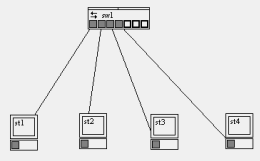
\includegraphics[width=0.6\textwidth]{./object/g3.png}
	\caption{Configuration du réseau}
\end{figure}

Après avoir ajusté le niveau VLAN au niveau 1 on configure la table Port/VLAN de la façon suivante :

\begin{figure}[ht!]
	\begin{tabular}{|l|l|}
		\hline
		Port & Vlan \\
		\hline
		1    & 1    \\
		2    & 1    \\
		3    & 2    \\
		4    & 2    \\
		\hline
	\end{tabular}
	\caption{Table Port/VLAN}
\end{figure}

Lorsque \texttt{st2} émet un broadcast sur le réseau que les appareils sur VLAN de niveau 1 peuvent le recevoir.

Quand on change le niveau du switch on s'aperçoit que les transmission ne change pas. 


\begin{dent}{Q2 :}
	\begin{figure}[ht!]
		\centering
		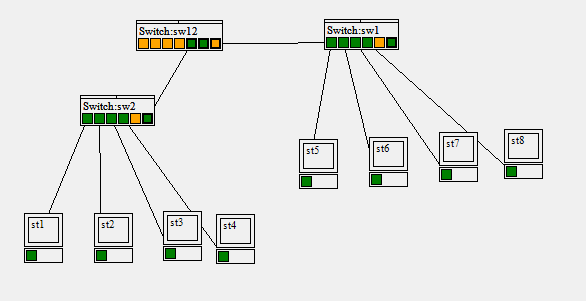
\includegraphics[width=0.7\textwidth]{./object/g5.png}
		\caption{Configuration du réseau}
	\end{figure}
	
\end{dent}



\end{document}
